\begin{figure}[t]
\centering
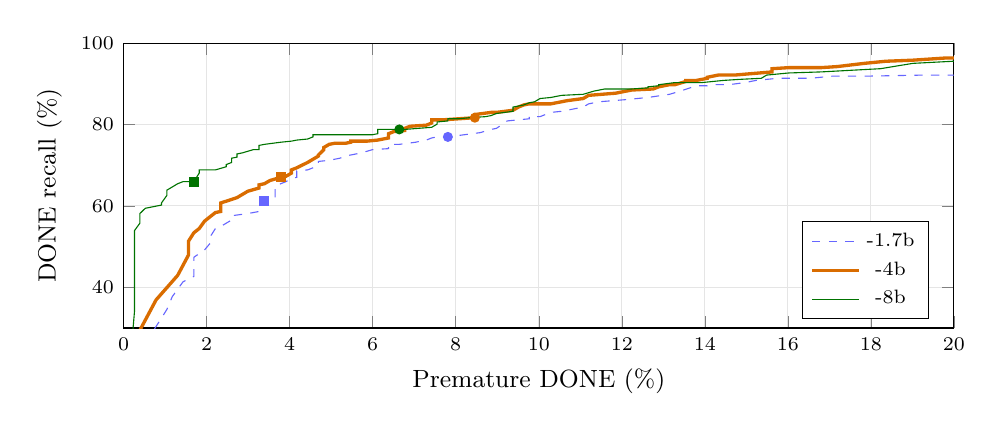
\begin{tikzpicture}
\begin{axis}[width=\linewidth, height=5.2cm, xlabel={Premature DONE (\%)}, ylabel={DONE recall (\%)},
  xmin=0, xmax=20, ymin=30, ymax=100, grid=major, grid style={gray!20}, legend pos=south east,
  legend style={font=\scriptsize}, tick label style={font=\scriptsize}, label style={font=\small}]
\addplot[color=blue!60, dashed] coordinates {(37.63,97.12) (34.90,97.12) (32.68,97.12) (30.47,96.07) (28.39,95.03) (27.08,95.03) (26.56,94.76) (25.78,94.24) (25.39,93.46) (24.48,92.93) (23.57,92.67) (22.92,92.67) (22.53,92.67) (21.88,92.41) (20.44,92.15) (19.27,92.15) (17.84,91.88) (17.06,91.88) (16.54,91.36) (15.76,91.36) (15.23,90.84) (14.97,90.31) (14.58,89.79) (14.19,89.79) (14.06,89.53) (13.80,89.53) (13.41,88.22) (13.15,87.43) (12.63,86.65) (12.11,86.13) (11.46,85.60) (11.46,85.60) (11.20,85.08) (11.07,84.29) (10.81,83.77) (10.55,83.25) (10.29,82.98) (10.03,81.94) (9.77,81.94) (9.77,81.41) (9.24,80.89) (8.98,79.06) (8.85,78.80) (8.59,78.01) (8.20,77.49) (7.81,76.96) (7.55,76.96) (7.42,76.70) (7.42,76.70) (7.29,76.18) (7.16,75.92) (7.03,75.65) (6.64,75.13) (6.38,75.13) (6.38,74.08) (5.99,73.82) (5.73,73.04) (5.34,72.25) (5.21,71.73) (5.21,71.73) (4.95,71.20) (4.69,70.94) (4.69,70.42) (4.69,69.90) (4.56,69.37) (4.43,68.85) (4.17,68.59) (4.17,67.02) (4.04,66.75) (3.91,65.97) (3.65,64.92) (3.65,63.61) (3.65,63.35) (3.65,62.83) (3.65,62.04) (3.39,61.26) (3.39,59.95) (3.26,58.64) (2.99,58.12) (2.60,57.59) (2.60,56.54) (2.34,54.97) (2.21,54.45) (2.08,52.36) (2.08,50.79) (1.95,49.21) (1.69,47.38) (1.69,45.55) (1.69,42.67) (1.43,41.36) (1.17,37.70) (1.04,34.55) (0.65,28.27) (0.39,19.11) (0.00,9.16)};
\addlegendentry{\wev-1.7b}
\addplot[color=orange!85!black, very thick] coordinates {(25.39,97.91) (23.70,97.38) (22.66,96.60) (20.83,96.34) (19.79,96.34) (19.01,95.81) (18.36,95.55) (17.84,95.03) (17.19,94.24) (16.80,93.98) (16.02,93.98) (15.62,93.72) (15.62,92.93) (14.71,92.15) (14.32,92.15) (14.19,91.88) (14.06,91.62) (14.06,91.62) (14.06,91.62) (14.06,91.36) (13.80,90.84) (13.54,90.84) (13.54,90.58) (13.28,89.79) (13.15,89.79) (13.15,89.79) (12.89,89.27) (12.76,88.74) (12.76,88.74) (12.76,88.74) (12.24,88.48) (11.98,87.96) (11.85,87.70) (11.20,87.17) (11.07,86.39) (10.68,85.86) (10.29,85.08) (9.77,85.08) (9.64,84.82) (9.51,84.29) (9.51,84.29) (9.38,83.51) (8.98,82.98) (8.85,82.98) (8.46,82.46) (8.46,81.68) (7.68,81.15) (7.42,81.15) (7.42,80.37) (7.29,79.84) (6.90,79.58) (6.77,79.06) (6.77,78.80) (6.77,78.53) (6.51,78.27) (6.38,77.75) (6.38,76.70) (6.12,76.18) (5.86,75.92) (5.60,75.92) (5.47,75.92) (5.47,75.65) (5.34,75.39) (5.21,75.39) (5.08,75.39) (4.95,75.13) (4.82,74.35) (4.82,73.82) (4.69,72.51) (4.69,72.25) (4.43,70.68) (4.17,69.37) (4.04,68.85) (4.04,68.06) (3.91,67.28) (3.78,67.02) (3.52,66.23) (3.39,65.45) (3.26,65.18) (3.26,64.40) (2.99,63.61) (2.73,62.04) (2.34,60.73) (2.34,59.42) (2.34,58.64) (2.21,58.38) (1.95,56.28) (1.82,54.45) (1.69,53.40) (1.56,51.31) (1.56,47.91) (1.30,42.93) (0.78,36.91) (0.26,26.96) (0.00,14.14)};
\addlegendentry{\wev-4b}
\addplot[color=green!45!black] coordinates {(22.27,96.86) (20.96,96.07) (19.01,95.03) (18.23,93.72) (16.80,92.93) (16.02,92.67) (15.49,92.15) (15.36,91.36) (14.84,91.10) (14.45,90.84) (13.93,90.31) (13.54,90.31) (13.28,90.31) (12.89,89.79) (12.89,89.53) (12.63,89.27) (12.63,89.01) (12.24,88.74) (11.98,88.74) (11.59,88.74) (11.33,88.22) (11.07,87.43) (10.55,87.17) (10.29,86.65) (10.03,86.39) (9.90,85.60) (9.77,85.34) (9.64,84.82) (9.38,84.29) (9.38,84.03) (9.38,83.77) (9.38,83.25) (8.98,82.72) (8.85,82.20) (8.72,81.94) (8.33,81.68) (8.07,81.41) (7.81,81.41) (7.81,80.89) (7.55,80.63) (7.55,80.37) (7.55,80.10) (7.42,79.32) (6.77,78.80) (6.64,78.80) (6.64,78.80) (6.64,78.80) (6.12,78.80) (6.12,77.75) (5.99,77.49) (5.60,77.49) (5.47,77.49) (4.95,77.49) (4.56,77.49) (4.56,76.96) (4.43,76.44) (4.17,76.18) (4.04,75.92) (3.78,75.65) (3.78,75.65) (3.39,75.13) (3.26,74.87) (3.26,74.61) (3.26,73.82) (3.12,73.82) (2.86,73.04) (2.73,72.77) (2.73,71.99) (2.60,71.73) (2.60,70.68) (2.47,70.16) (2.47,69.63) (2.21,68.85) (1.82,68.85) (1.82,68.06) (1.69,65.97) (1.43,65.97) (1.30,65.45) (1.30,65.45) (1.04,63.87) (1.04,63.35) (1.04,62.57) (0.91,60.73) (0.91,60.21) (0.52,59.42) (0.39,58.12) (0.39,57.59) (0.39,55.76) (0.26,53.93) (0.26,51.05) (0.26,47.12) (0.26,44.76) (0.26,40.84) (0.26,34.03) (0.13,18.32)};
\addlegendentry{\wev-8b}
\addplot[only marks, mark=*, mark size=1.6pt, color=blue!60, forget plot] coordinates {(7.81,76.96)};
\addplot[only marks, mark=square*, mark size=1.6pt, color=blue!60, forget plot] coordinates {(3.39,61.26)};
\addplot[only marks, mark=*, mark size=1.6pt, color=orange!85!black, forget plot] coordinates {(8.46,81.68)};
\addplot[only marks, mark=square*, mark size=1.6pt, color=orange!85!black, forget plot] coordinates {(3.78,67.02)};
\addplot[only marks, mark=*, mark size=1.6pt, color=green!45!black, forget plot] coordinates {(6.64,78.80)};
\addplot[only marks, mark=square*, mark size=1.6pt, color=green!45!black, forget plot] coordinates {(1.69,65.97)};
\end{axis}
\end{tikzpicture}
\caption{Stopping trade-off on the NNetNav test split (382 DONE steps, 768 others). Each curve
accepts DONE only when its probability exceeds a threshold swept from 0.05 to 0.99; circles mark 0.5 and squares 0.8.}
\label{fig:done}
\end{figure}
\newcommand{\DONECURVETEXT}{At a threshold of 0.5, \wev-4b recalls 82\% of DONE steps and stops early on 8.5\% of the others; at 0.8 the premature rate falls to 3.8\% while recall falls to 67\%. \wev-8b reaches 1.7\% premature stops at 66\% recall, or 2.9\% at 73\% with a threshold of 0.7. The curves are smooth, so a deployment can choose its operating point from development data rather than accept the most probable operation, which answers DONE whenever it outranks the other seven operations and so behaves like a threshold below 0.5.}
